%----------------------------------------------------------------------------------------
%	PACKAGES AND OTHER DOCUMENT CONFIGURATIONS
%----------------------------------------------------------------------------------------

\documentclass[DIV=calc, paper=a4, fontsize=11pt, twocolumn]{scrartcl}	 % A4 paper and 11pt font size

\usepackage[english]{babel} % English language/hyphenation
\usepackage[protrusion=true,expansion=true]{microtype} % Better typography
\usepackage{amsmath,amsfonts,amsthm} % Math packages
\usepackage[svgnames]{xcolor} % Enabling colors by their 'svgnames'
\usepackage[hang, small,labelfont=bf,up,textfont=it,up]{caption} % Custom captions under/above floats in tables or figures
\usepackage{booktabs} % Horizontal rules in tables
\usepackage{fix-cm}	 % Custom font sizes - used for the initial letter in the document
\usepackage[pdftex]{graphicx}     
\usepackage{hyperref}

\usepackage{sectsty} % Enables custom section titles
\allsectionsfont{\usefont{OT1}{phv}{b}{n}} % Change the font of all section commands

\usepackage{fancyhdr} % Needed to define custom headers/footers
\pagestyle{fancy} % Enables the custom headers/footers
\usepackage{lastpage} % Used to determine the number of pages in the document (for "Page X of Total")
\usepackage{hyperref}

% Headers - all currently empty
\lhead{}
\chead{}
\rhead{}

% Footers
\lfoot{}
\cfoot{}
\rfoot{\footnotesize Page \thepage\ of \pageref{LastPage}} % "Page 1 of 2"

\renewcommand{\headrulewidth}{0.0pt} % No header rule
\renewcommand{\footrulewidth}{0.4pt} % Thin footer rule

\usepackage{lettrine} % Package to accentuate the first letter of the text
\newcommand{\initial}[1]{ % Defines the command and style for the first letter
\lettrine[lines=3,lhang=0.3,nindent=0em]{
\color{DarkGoldenrod}
{\textsf{#1}}}{}}

%----------------------------------------------------------------------------------------
%	TITLE SECTION
%----------------------------------------------------------------------------------------

\usepackage{titling} % Allows custom title configuration

\newcommand{\HorRule}{\color{DarkGoldenrod} \rule{\linewidth}{1pt}} % Defines the gold horizontal rule around the title

\pretitle{\vspace{-30pt} \begin{flushleft} \HorRule \fontsize{50}{50} \usefont{OT1}{phv}{b}{n} \color{DarkRed} \selectfont} % Horizontal rule before the title

\title{Evolutionary Game Theory} % Your article title

\posttitle{\par\end{flushleft}\vskip 0.5em} % Whitespace under the title

\preauthor{\begin{flushleft}\large \lineskip 0.5em \usefont{OT1}{phv}{b}{sl} \color{DarkRed}} % Author font configuration

\author{Elena Rosskopf and Ellen Halaburt, } % Your name

\postauthor{\footnotesize \usefont{OT1}{phv}{m}{sl} \color{Black} % Configuration for the institution name
Module Evolutionary Game Theory WS 2014/15 % Your institution

\par\end{flushleft}\HorRule} % Horizontal rule after the title

\date{\today} % Add a date here if you would like one to appear underneath the title block

%----------------------------------------------------------------------------------------

\begin{document}

\maketitle % Print the title

\thispagestyle{fancy} % Enabling the custom headers/footers for the first page 

%----------------------------------------------------------------------------------------
%	ABSTRACT
%----------------------------------------------------------------------------------------

% The first character should be within \initial{}
\initial{U}\textbf{nderstanding, estimating and forecasting social dilemmas via modelling is a crucial part of theoretical ecology nowadays. Evolutionary game theory plays a major role in trying to understand and model the theory of cooperation evolving via natural selection. Constructing such cooperation models in a simple way can be done in two basic and known games, the Prisoner's Dilemma (PD) and the Snowdrift game (SD). Both games are two person-player games with two strategies (2x2) and both are social dilemmas, meaning that cooperators are exploited by defectors. Cooperation does normally not persist in PD, but can evolve to maintain in SD at moderate proportion. Here, we investigate the functioning of those games in different scenarios. The first one will be generally held as individuals from a non-spatial, well-structured population will play against each other. The second scenario will focus on the spatial structure with the implementation of different neighbourhood structures, keeping pure strategies either cooperation or defection. The last scenario will give insights in the option of each individual inheriting a mixed strategy probability. }\\

Looking at the evolutionary game structures, the pay-off is crucial to determine each players fitness and the fitness of a whole group. We will further investigate the differences of the games pay-off matrices and the subsequent changes in behaviour of the individuals in the game. \\

Spatial structure added to the game results in a population, where its individuals occupy patches on a spatial lattice (here two dimensional). 
Each tick (update) will be done by letting individuals play against their nearest neighbours. The resulting pay-offs will be used to decide upon the focal patch's future occupant. It could be an offspring of the last occupant resisting the invasion or from a neighbour spreading its strategy. The lattice is updated and the evolutionary process takes place with every update.

%----------------------------------------------------------------------------------------
%	ARTICLE CONTENTS
%----------------------------------------------------------------------------------------


\subsection*{Prisoners Dilemma}

In the PD, the cooperators get exploited by defectors, subsequently defectors are naturally selected. The cost to the donor of fitness(pay-off?) is always higher than zero, but generally lower the benefit to the receiver of the pay-off ( $b > c > 0 $). The defector's pay-off is the highest pay-off b if the other player is cooperating. The lowest pay-off, namely only the cost, has then (-c) the cooperator which is defected in the unilateral cooperation. Finally it is best to defect regardless of other players decision. Mutual defections result then in pay-off zero for both players, not reducing the fitness but also not increasing it (see \ref{table1}). Here, the defector strategy is the ESS. 

\begin{table}[h]
\caption{Prisoner's Dilemma}
\label{table1}
\centering
\begin{tabular}{lll}
%\toprule
%\multicolumn{2}{c}{Name} \\
%\cmidrule(r){1-2}
 & C & D \\
\midrule
Payoff to C & $b-c$ & $-c$ \\
Payoff to D & $b$ & $0$ \\
\bottomrule
\end{tabular}
\end{table}

Spatial structure in Prisoners Dilemma is a potent promoter of cooperation. Cooperators stay on forming large compact clusters thus reducing the exploitation by defectors as one can see in figure \ref{fig:PDspatialcluster}. In this case the cooperators are not close to the threshold of extinction and survive in big clusters. 

The difference to non-spatial PD is, that cooperation can evolve as a stable proportion in the population, which would be not possible without the spatial component in the behaviour. 

\begin{figure}[here]
\centering
\begin{minipage}{.35\textwidth}
  \centering
  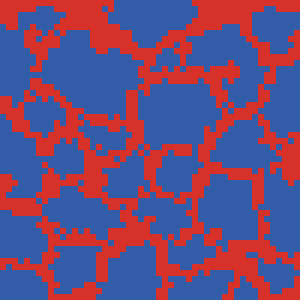
\includegraphics[width=1\linewidth]{PDspatial8cost01}
 \caption{Clustering of cooperators in spatial PD with b=1, c=0.1, N=8, blue=C, red=D}
\label{fig:PDspatialcluster}
\end{minipage}%
\end{figure}

\begin{figure}
\begin{minipage}{.48\textwidth}
  \centering
  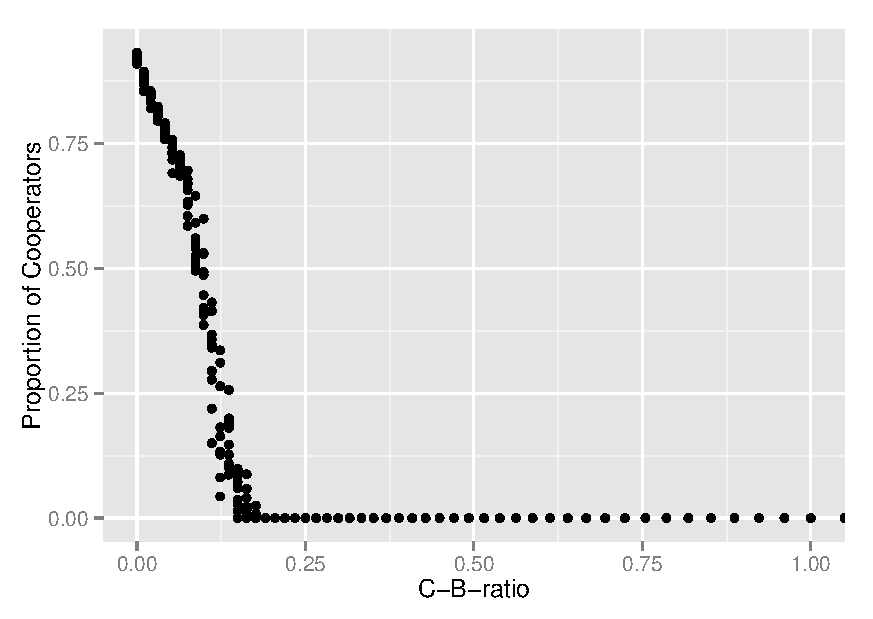
\includegraphics[width=1\linewidth]{spatialPDratio}
 \caption{Frequency of cooperators against c-b-ratio, N=8}
  \label{fig:PDspatialfreq}
\end{minipage}
\end{figure}
%------------------------------------------------

\subsection*{Snowdrift game}

In the snowdrift game we face some differences to Prisoners Dilemma. The players can share the benefit and the cost, depending on their strategies. Another feature in this game is, that if one defects, the pay-off could be less than the sucker's pay-off of the unilateral cooperator. Still defecting if the other player cooperates is, according to the matrix, the best response choice. The other way round, if the opponent defects, it is still better to cooperate than to defect also. This leads to the maintenance of cooperation to a certain extent in the population as an ESS. As one can see in table \ref{table2}, the pay-off matrix is slightly different than the one of Prisoners Dilemma in table \ref{table1}. 
If $2b > c > b > 0$, meaning that if costs are high, these pay-off structures change the game to a PD and affect the reverse pay-off structure. If $b > c > 0$ , the best action depends on co-players action resulting in a mixed strategy population, where rare strategies can invade, either defector or cooperator with an ESS at cooperator proportion is $1- c/(2b-c)$. Here it gets important to investigate when the cooperation in the ESS is increased or decreased.


\begin{table}[h]
\caption{Snowdrift game}
\label{table2}
\centering
\begin{tabular}{lll}
%\toprule
%\multicolumn{2}{c}{Name} \\
%\cmidrule(r){1-2}
 & C & D \\
\midrule
Payoff to C & $b-c/2$ & $b-c$ \\
Payoff to D & $b$ & $0$ \\
\bottomrule
\end{tabular}
\end{table}

In comparison to the spatial structure  of the Prisoner's Dilemma's resulting cooperation lattice, the cooperators form only small filament-like clusters in the snowdrift game. The defectors have via the isolated cooperators structure the advantage to exploit them and break in those fragile clusters. They can invade due to the pay-off matrix and the aim of developing a strategy contrary to the neighbour one. The isolated cooperators can develop branchy structures but never evolve to large communities in the snowdrift game. 

\begin{figure}[here]
\centering
\begin{minipage}{.35\textwidth}
  \centering
  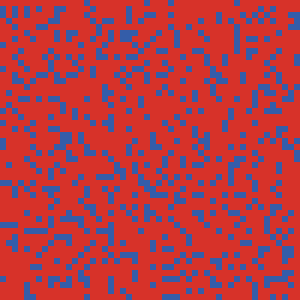
\includegraphics[width=1\linewidth]{HDspatial06neu}
 \caption{Clustering of cooperators in spatial SD, c-b-ratio=0.6}
\label{fig:PDspatialcluster}
\end{minipage}%
\end{figure}

The individuals occupy patches on a regular lattice. The next update is done by populating this patch with the offspring. Which offspring depends on the game result of the present occupant and its nearest neighbour competing for the site. The competitive success depends therefore on the different pay-off that each player and possible parent gains from game interactions. 

But after several updates spatial structure seems to fail to enhance cooperation in the snowdrift game. In moderate c-b-ratios, cooperation is actually proportionally lower than in non-spatial populations, what is a difference to the behaviour of players in spatial PD. 

A small ratio, meaning high benefits with low costs can increase the proportion of cooperation compared to non-spatial populations. The frequency is higher than the $1-r$ expected frequency in well-mixed populations. If the costs are increasing and the c-b-ratio is high, the defectors have an advantage and their proportion increase, making spatial structuring not always beneficial for cooperators. 

Cooperation is lost if sufficiently high ratio and disappears when the ratio is $1/N > 1- r$, which you can see in the next chapter as different N ( neighbourhood structures) are applied. 




%------------------------------------------------

\section*{The experiments}

First we conducted two experiments to check the validity of our implementation.
The first one runs 50 experiments with benefit 1 and cost 1.5. According to the paper of Hauert and Doebli (cite) this should result in a fast domination of defectors. The second experiment used benefit 1 and cost .75. This results in a stable distribution of defectors and cooperators. Both results could be achieved. It was important to check the plausibility of the experiment, especially to gain certainty that the equilibrium is stable and the variation will not change again. The verification, when to stop the calculations and repetitions was done via statistical testing (for detailed information see appendix).
The second experiment can be visualized in further figures, with a stable average of 24,7\% cooperators in the population as an ESS. \\

\begin{figure}[here]
\centering
\begin{minipage}{.48\textwidth}
  \centering
  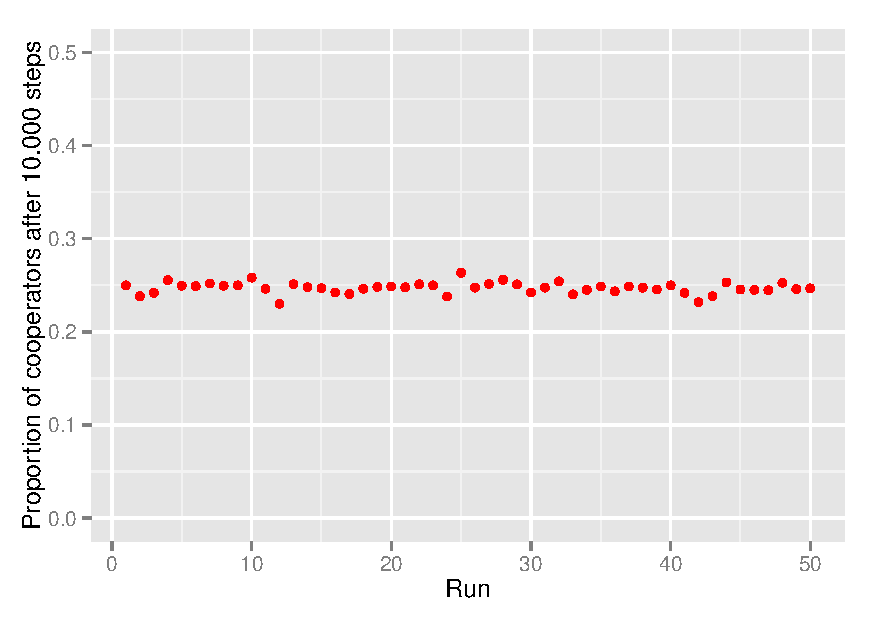
\includegraphics[width=1\linewidth]{task1prop}
 \caption{Proportion of cooperators in the population after 10000 steps}
\label{fig:PDspatialcluster}
\end{minipage}%
\end{figure}
%-------------

\begin{figure}[here]
\centering
\begin{minipage}{.48\textwidth}
  \centering
  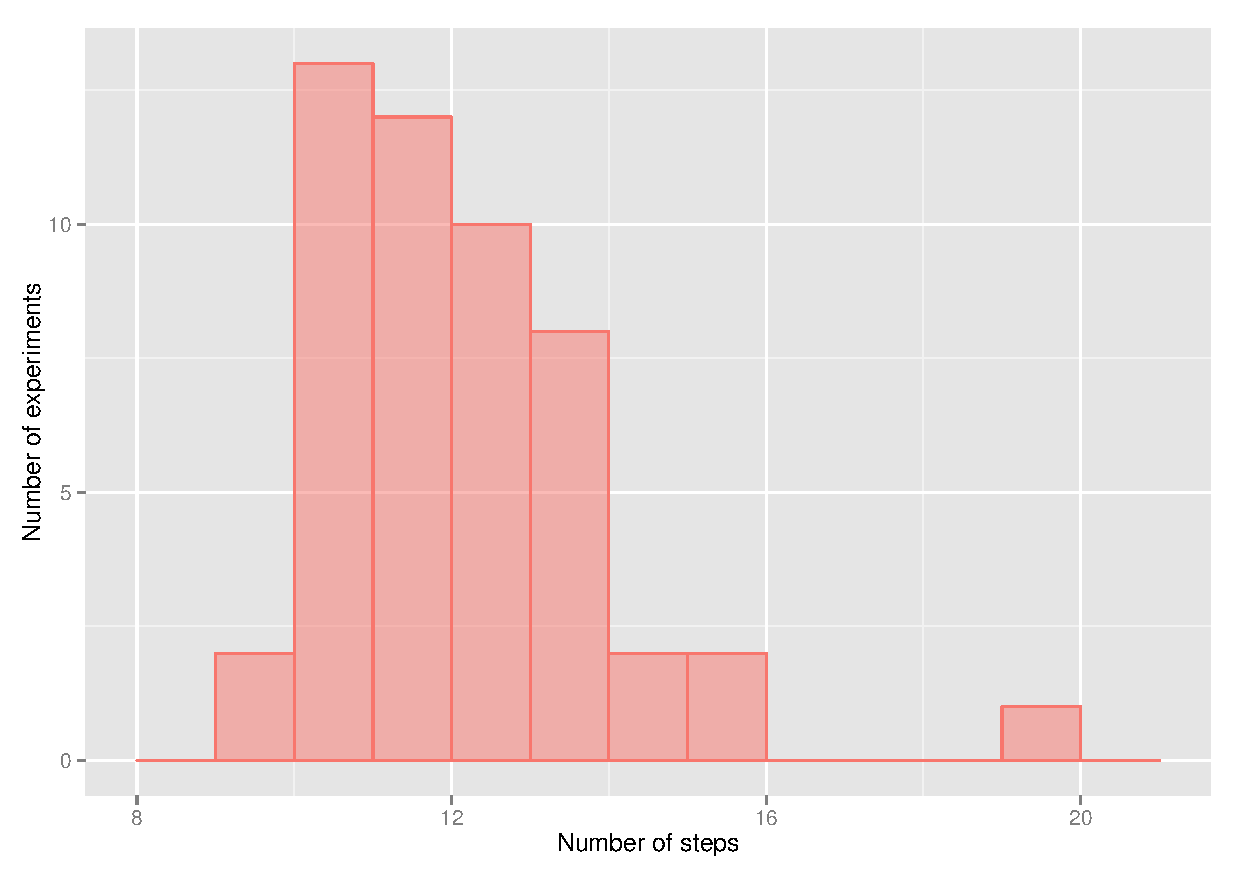
\includegraphics[width=1\linewidth]{task1numberofexstep}
 \caption{Histogram: Number of experiments against number of steps}
\label{fig:histo}
\end{minipage}%
\end{figure}


\section*{The neighbourhood problem}

We choose 3 different types of neighbourhoods to be experimented on. The first one is the Moore neighbourhood with the default value of N=8 neighbours. The neighbours surround the focal patch in 8 directions. The second neighbourhood is the Von Neumann neighbourhood with the default value of N=4 neighbours which are orthogonally surrounding the focal patch on a two dimensional square lattice. The last type of neighbourhood introduces a parameter instead of a defined neighbourhood, having the attribute of a radius equal or less than 3 patches surrounding the focal patch. \\
To increase the certainty of our results, the behaviour space model is used to compare different cooperation frequencies against the ratio of cost and benefit within different neighbourhood features and between the snowdrift game and the prisoners dilemma game. \\
The mutual cooperation ratio in the snowdrift game is calculated as $r = c / (2b-c)$ , cost to benefit ratio. The mutual cooperation ratio in the Prisoner's Dilemma is calculated as $r = c/ (b-c) $.\
If one applies the Hamilton's rule to spatial PD with differing neighbours, the general assumption of $r = c / (b-c) $ must be improved with the rule that cooperators can invade if $ b - n * c > 0$ and if $ r = 1/N $. In the experiment of the neighbourhood structure of Moore (cite) with 8 neighbours, it would mean, that the ratio needs to be higher than 0.125 ( $b > 8c$, $ r = c/(b-c) < 0.125$) what you can see in the plots of figure \ref{fig:PDspatialfreq}. 

With the different neighbourhood interactions in this experiment, the cooperator proportion is always rather small. The probability that the neighbours are related to the invading cooperator is small, the neighbours tend to be defectors. 

The different neighbourhood experiments verify the Hamilton's rule (cite), as the threshold of an ESS favouring cooperators corresponds roughly to the calculations given above. It is thus possible to change the defecting ESS by adding a spatial structure to the PD. \\

\begin{figure}[here]
\centering
\begin{minipage}{.35\textwidth}
  \centering
  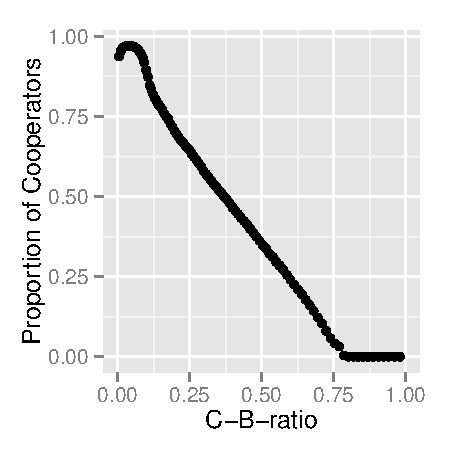
\includegraphics[width=1\linewidth]{HDN8}
 \caption{N=8}
\label{fig:HDm1}
\end{minipage}%
\end{figure}

\begin{figure}[here]
\centering
\begin{minipage}{.35\textwidth}
  \centering
  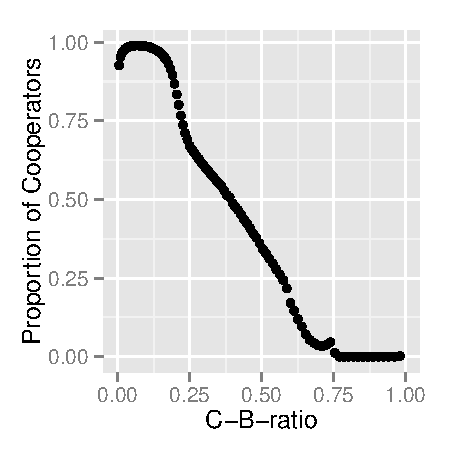
\includegraphics[width=1\linewidth]{HDN4}
 \caption{N=4}
\label{fig:HDn1}
\end{minipage}%
\end{figure}

\begin{figure}[here]
\centering
\begin{minipage}{.35\textwidth}
  \centering
  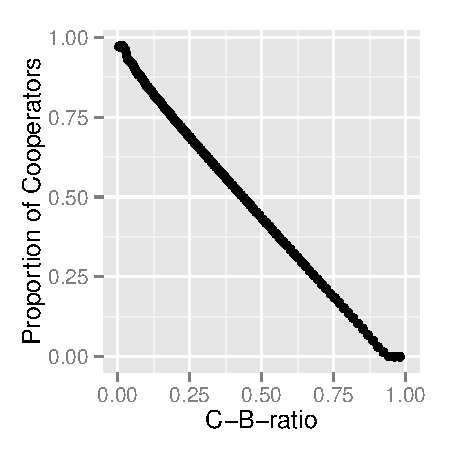
\includegraphics[width=1\linewidth]{HDN3}
 \caption{N=3}
\label{fig:HDm3}
\end{minipage}%
%\end{figure}
\end{figure}

The spatial structure results of the snowdrift game concerning the c-b-ratio have very contrary effects on cooperation proportion compared to the spatial PD experiments. With increasing neighbours, the proportion of cooperators is decreasing faster than expected. The expected frequency 1-r is roughly consistent with the last neighbourhood experiment of having N=3 in figure \ref{fig:HDm3}.  \\

\section*{The mixed strategy}

After checking different options in the spatial structure of a snowdrift game, we can also check for mixed strategies. In the last chapters, the strategies were purely either cooperation or defection. The mixed strategies implementation gives each player a probability $p$ to play $cooperation$ in the next update. This probability is heritable and subject to a mutation rate where the probability is slightly increased or decreased. \\



\subsection*{The Algebra of the Nash Equilibrium}

The simulation for the third task ended in a Nash Equilibrium
for the snow drift game. In order to verify the result of our
simulation we will derive the probability for the mixed strategy
for the ``defector player''.

The pay-off matrix for the snowdrift game is calculated as follows:\\

\begin{tabular}{l|ll}
  & Left & Right \\
\midrule
Up & $b-(c/2)$ & $b-c$ \\
Down & $b$ & $0$ \\
\end{tabular}

We simulated the game for benefit $b=1$ and cost $c=0.75$.
So the actual pay-off matrix is:\\

\begin{tabular}{l|ll}
  & Left & Right \\
\midrule
Up & $0.625$ & $0.25$ \\
Down & $1$ & $0$ \\
\end{tabular}

Let $\sigma$ be the probability for the mixed strategy
to play $C$ and let $U_x$ be the utility function for the
player when playing strategy ``Left'' ($L$) or ``Right'' ($R$)
respectively. We get the equation system:
\begin{align*}
  U_L &= U_R\\
  U_L &= f(\sigma)\\
  U_R &= f(\sigma)
\end{align*}

We can further define (this is just the probability
of the strategy multiplied with the payoff, for both
strategies):
\begin{align*}
  U_L &= 0.625\sigma + 1 \cdot (1-\sigma)\\
  U_R &= 0.25\sigma + 0 \cdot (1-\sigma)
\end{align*}

Set the two equations for $U_L = U_R$, we get:
\begin{align*}
0.625\sigma + (1-\sigma) =  0.25\sigma
\end{align*}

The resulting $\sigma$ is $0.60$. 

The real value of the equilibrium is with 99\% probability between 0.596188 and 0.5965448. Both will be rounded to 0.60. The standard deviation is also relatively small being $sd = 0.01234907$. Also the summary in the table below is strengthening the integrity of the model. This is converging with the theory behind our modelling with the calculated sigma above, thus assuming that theory and practice are consistent. \\
 
\begin{minipage}{.42\linewidth}
\begin{tabular}{llllll}
  Min. & 1st Q. & Median  &  Mean& 3rd Q.  &  Max.  \\
\midrule
.542 & .588 & .596&  .596 & .605 & .647 \\
%\caption{Summary of the Nash equilibrium focusing on defectors}
\end{tabular}
\end{minipage}

\begin{figure}[here]
%\begin{minipage}{.48\textwidth}
  \centering
  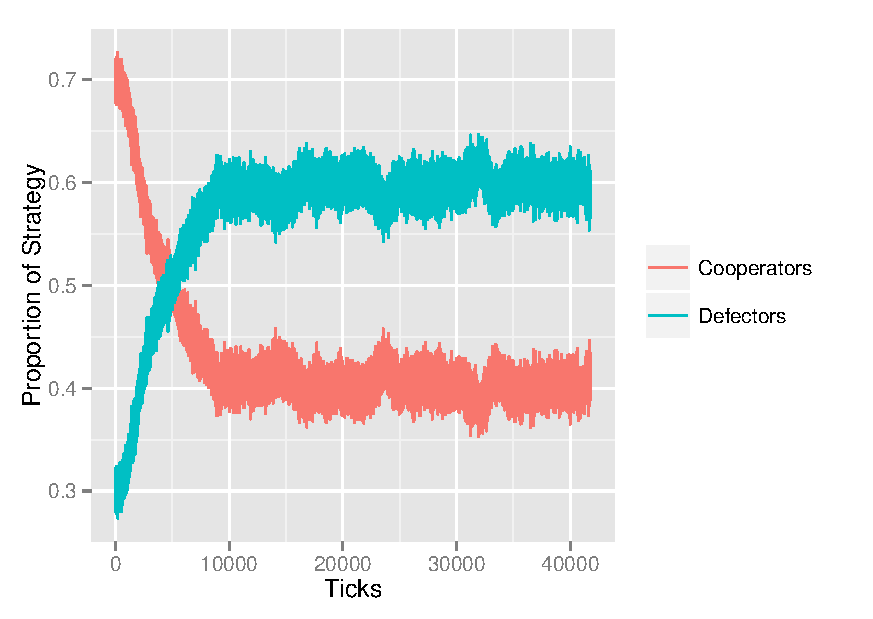
\includegraphics[width=1\linewidth]{task3}
 \caption{Resulting evolution in a mixed strategy snowdrift game}
\label{fig:task3}
%\end{minipage}%
\end{figure}

\section*{discussion}



where can we give in more time, where are options to prolong this topic? relation to nature, where is the importance here ? 

Discussion: 
Paper: http://iopscience.iop.org/0253-6102/57/4/04
Not included the noise, like in this paper  - could it make even more realistic but heavier to implement
Our study more straighforward to understand the snowdrift game and the players evolution better
Afterwards you could add those noise to our model to make it more exact

"Some analytical results have been obtained using geometrical arguments about cluster formation (Nowak \& May 1992; Killingback et al. 1999; Hauert 2001), and Schweitzer et al. (2002) recently gave a classification of the dynamic regimes in the spatial PD."

http://www.math.pitt.edu/~bard/classes/mth3380/spatialgame.pdf

continuous spatial SD - change of function of cost and benefit ( investment) leading somehow to the tragedy of commune as contrast to tragedy of commons 

tragedy of commons in PD: cooperation will be advantageous only for others, elimination of altruism 
tragedy of commune in SD: coop system, all individuals contribute to group benefit, but option to asymmetric stable state where some invest a lot and others less or nothing: stichwort fairness, diversification

PD and SD both social dilemma
PD spatial assortment crucial for coop, where defectors dominant
SD spatial assortment irrelevant, coop can invade if rare

all experiments are very theoretically and neglecting a lot of ecological dynamics and parameters which are important for evolution in reality
missing input of empirical studies, raw data


\section*{Appendix - the plausibility verification}
\label{sec:appendix}
\noindent We were determining whether first 1000, then 500 steps are sufficient for reaching a rather stable state with the two-sided t-test and the F-test to compare two variances of the different final proportions of cooperators (the final proportion and the proportion of cooperators after 1000 and 500 updates, respectively). \\

\begin{tabular}{l|ll}
\centering
  & p-value & NULL hyp \\
\midrule
F-Test & $>0.05$ & $accepted$ \\
t-test & $>0.05$ & $accepted$ \\
\end{tabular}

\noindent Also we tested whether the initial proportion of defectors has some impact on the final cooperation proportion with a starting value of 0.4 and 0.6. The tests confirmed the NULL hypotheses that variances are the same and there is no difference in means between the two possible initial defector proportions. So we can assume that if cost and benefit structures are given, the stable distribution of the final cooperation proportion is evolving. 


\nocite{Albizu2013}
%----------------------------------------------------------------------------------------
%	REFERENCE LIST
%----------------------------------------------------------------------------------------
\bibliography{literatur}
\bibliographystyle{plain}

%----------------------------------------------------------------------------------------

\end{document}
